\section{Motivaci�n}

\subsection{Presentaci�n del problema b�sico}
\begin{frame}
	\frametitle{�C�mo detectar patrones de enfermedades de la piel?}
	\begin{itemize}
		\item �C�mo detectar patrones de enfermedades de la piel?
		\item Resultan naturales y poco complejos para un ser humano
		\item �Y para un ordenador?
	\end{itemize}
\end{frame}

\subsection{Ejemplos}
\begin{frame}
	\frametitle{Ejemplo: Dos enfermedades}
	\begin{tabular}{cc}
		Varicela & 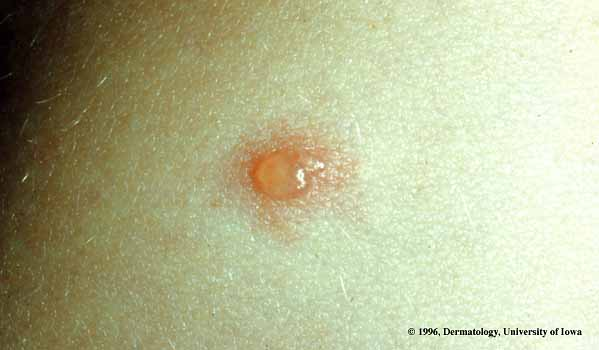
\includegraphics[width=2in]{../Imagenes/U.Iowa/Varicel-02.jpg} \\
		Sarampi�n & 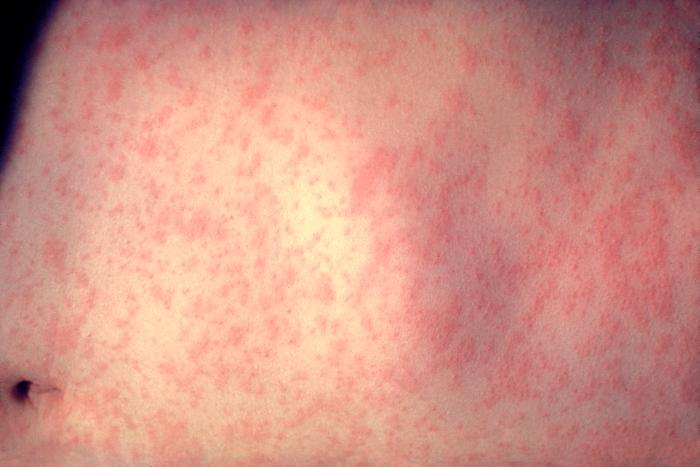
\includegraphics[width=2in]{../Imagenes/U.Iowa/measles-PHIL_3168_lores.jpg} \\
	\end{tabular}
\end{frame}

\begin{frame}
	\frametitle{Ejemplo: Variabilidad de im�genes para una misma enfermedad}
	\begin{tabular}{ cc }
		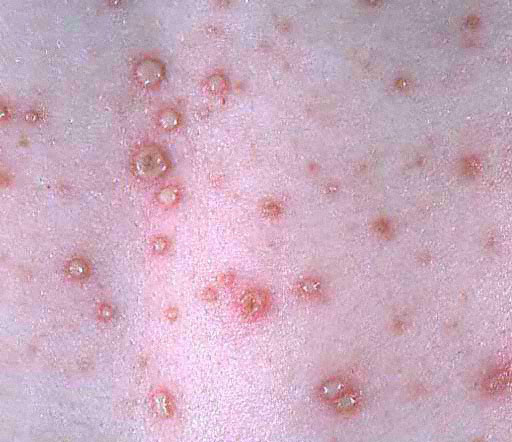
\includegraphics[width=1.6in]{../Imagenes/U.Iowa/chicken_pox_picture_13.jpg} & 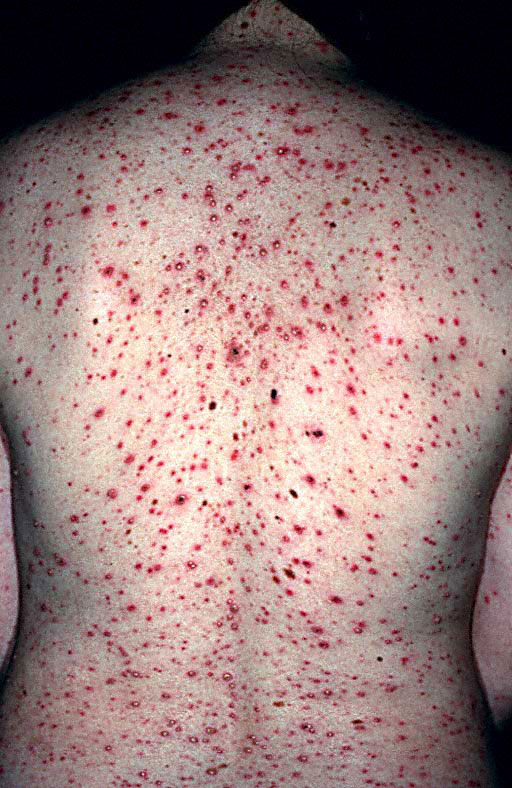
\includegraphics[width=0.9in]{../Imagenes/U.Iowa/chicken_pox_picture_01.jpg} \\
		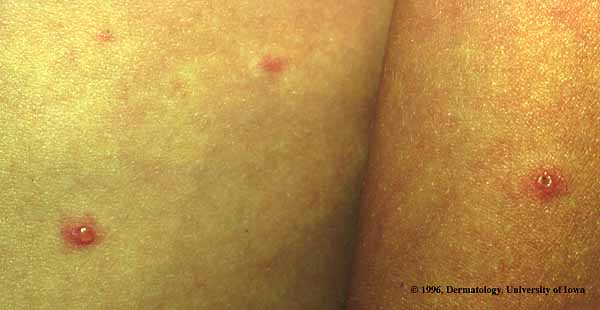
\includegraphics[width=1.6in]{../Imagenes/U.Iowa/Varicel-04.jpg} & 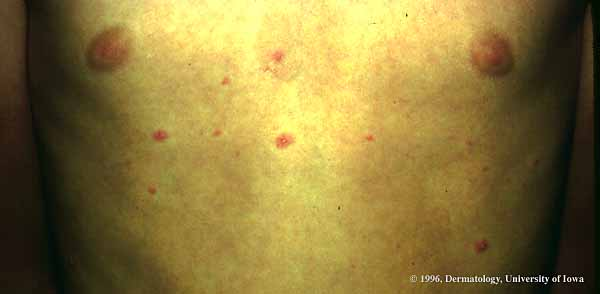
\includegraphics[width=1.6in]{../Imagenes/U.Iowa/Varicel-01.jpg} \\
	\end{tabular}
\end{frame}

% \subsection{Procesamiento digital de im�genes}
% \begin{frame}
	% \frametitle{Procesamiento digital de im�genes}
	% Este problema se enmarca en el procesamiento digital de im�genes.
	% Trabajos anteriores:
	% \begin{itemize}
		% \item ``An�lisis digital de im�genes en lesiones pigmentadas de la piel.\ Diagn�stico precoz del melanoma'' (Coll et al.\ 2007)
		% \item ``Pigmented skin lesions classification using dermatoscopic images'' (Capdehourat, Mus� et al.\ 2009)
		% \item ``Detecci�n estable de los bordes de la oreja en im�genes 2D'' (Flores y M�ndez, 2009)
		% \item ``Detecci�n del ojo de una persona y medici�n del iris'' (Bianchetti y Comastri, 2008, Terissi et al., 2000)
	% \end{itemize}
% \end{frame}
